
On peut dresser un arbre pondéré :
\begin{center}
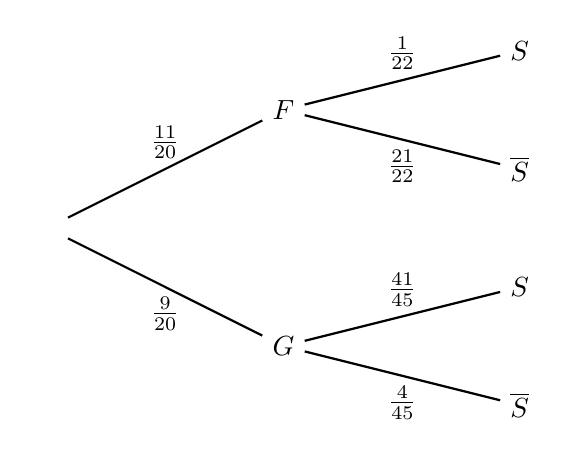
\begin{tikzpicture}[thick, scale=1.5]
\node (P_-1_0) at (-2,-1.5) {$\phantom{A}$};
\node (P_0_0) at (0,-0.5) {$F$};
\draw (P_-1_0) -- (P_0_0) node[midway, above] {$\frac{11}{20}$};
\node (P_1_0) at (2,-0) {$S$};
\draw (P_0_0) -- (P_1_0) node[midway, above] {$\frac{1}{22}$};
\node (P_1_1) at (2,-1) {$\overline{S}$};
\draw (P_0_0) -- (P_1_1) node[midway, below] {$\frac{21}{22}$};
\node (P_0_2) at (0,-2.5) {$G$};
\draw (P_-1_0) -- (P_0_2) node[midway, below] {$\frac{9}{20}$};
\node (P_1_2) at (2,-2) {$S$};
\draw (P_0_2) -- (P_1_2) node[midway, above] {$\frac{41}{45}$};
\node (P_1_3) at (2,-3) {$\overline{S}$};
\draw (P_0_2) -- (P_1_3) node[midway, below] {$\frac{4}{45}$};
\end{tikzpicture}
\end{center}

\subsection*{1.}

\[
p(G) = 1 - p(F) = 1 - \dfrac{110}{110 + 90} = 1 - \dfrac{110}{200} = \dfrac{90}{200} = \dfrac{9}{20};
\]
\[
p(G \cap \overline{S}) = p(G) \times p_G(\overline{S}) = \dfrac{9}{20} \times \dfrac{4}{45} = \dfrac{9 \times 4}{4 \times 5 \times 5 \times 9} = \dfrac{1}{25};
\]
De même :
\[
p(F \cap \overline{S}) = p(F) \times p_F(\overline{S}) = \dfrac{11}{20} \times \dfrac{1}{22} = \dfrac{11 \times 1}{4 \times 5 \times 2 \times 11} = \dfrac{1}{40}.
\]
D'après la loi des probabilités totales :
\[
p(\overline{S}) = p(F \cap \overline{S}) + p(G \cap \overline{S}) = \dfrac{1}{40} + \dfrac{1}{25} = \dfrac{5}{200} + \dfrac{8}{200} = \dfrac{13}{200}.
\]

\subsection*{2.}

On a :
\[
p_{\overline{S}}(G) = \dfrac{p(\overline{S} \cap G)}{p(\overline{S})} = \dfrac{p(G \cap \overline{S})}{p(\overline{S})} = \dfrac{\dfrac{9}{20} \times \dfrac{4}{45}}{\dfrac{13}{200}} = \dfrac{\dfrac{1}{25}}{\dfrac{13}{200}} = \dfrac{8}{13}.
\]

\subsection*{3.}

On a :
\[
p(G \cap S) = 1 - p(G \cap \overline{S}) = 1 - \dfrac{1}{25} = \dfrac{24}{25},
\]
et :
\[
p(G) \times p(S) = \dfrac{9}{20} \times \dfrac{187}{200} = \dfrac{90}{187},
\]
donc :

\(p(G \cap S) \neq p(G) \times p(S)\) : les événements G et S ne sont pas indépendants.

